\subsection{Equations of lines and planes in 3-space}

\subsubsection{Equations of planes}

Consider the following equations:

\begin{center}
    \begin{tabular}{ | c | }
        \hline
        \textbf{Equations of planes in 3-space}             \\ \hline
        Point-normal: $a(x-x_0) + b (y-y_0) + c(z-z_0) = 0$ \\ \hline
        General Form: $ax + by + cz + d = 0$                \\ \hline
        Vector form: $n(r-r_0) = 0$                         \\
        or $(a; b; c)(x-x_0; y-y_0; z-z_0) = 0$             \\ \hline
    \end{tabular}
\end{center}

We note that in the equations above, $(a; b; c)$ is a vector perpendicular to the plane and $(x_0; y_0; z_0)$ is a
specific point on the plane.
Thus when we determine the equation of a plane we need to find, from the information
provided, a point on the plane and a vector perpendicular to the plane.

\subsubsection{Equations of lines}

Consider the following equations:

\[ L_n
\begin{cases} 
x = x_0 + at \\ 
y = y_0 + bt & -\infty < t < \infty \\ 
z = z_0 + ct \\
\end{cases} 
\]

This equation represents parametric line equations in 3D space alternatively, we can write this equation in the following vector form:

\begin{center}
$r = r_0 + vt ,$ $ -\infty < t < \infty$ \\
or $(x,y,z) = (x_0+y_0+z_0)+(a,b,c)t$ 
\end{center}


We note that in the equations above, $(a; b; c)$ is a vector parallel to the line and $(x_0; y_0; z_0)$ is a specific
point on the line.
Thus when we determine the equations of a line we need to find, from the information
provided, a point on the line and a vector parallel to the line.
The important point to notice here is that when we are finding the equation
of a plane we need a vector perpendicular to the plane, and when we are
finding the equations of a line we need a vector parallel to the line.


\subsection{Determining the properties of planes and methodologies to prove them}
\subsubsection{Finding out if the planes are parallel or perpendicular/Orthogonal to each other}
\textbf{Procedure for testing perpendicular/Orthogonality planes}\\
To get started in proving that the planes are perpendicular/orthogonal to each other. We need to find out our two $(a,b,c)$ vectors.
We take our two planes and find the $(a,b,c)$ vector of each plane. \\

With these two vectors work out if the dot product is = 0 or not. \\

Consider vectors $n,v$

Using this formula to calculate:

\begin{equation}
    \arccos{(\theta)}(\frac{u*v}{\| u\Vert \| v\Vert })
\end{equation}

we can deduct where dot product is:

$\left(n_1,\:\:\ldots ,\:\:n_k\right)\cdot \left(v,\:\:\ldots ,\:\:v_k\right)=\sum _{i=1}^kx_iy_i$ \\

If $\sum _{i=1}^kx_iy_i = $ 0, then the planes are perpendicular else if not 0, then the planes are not perpendicular. \\

\textbf{Procedure for testing parallel planes} \\

Consider the following plane equations:
\begin{center}
 $a_1x+b_1y+c_1z+d_1=0$ \\
 $a_2x+b_2y+c_2z+d_2=0$ \\
\end{center}

if 
\begin{center}
    $\frac{a_1}{a_2} = \frac{b_1}{b_2} = \frac{c_1}{c_2}$\\
\end{center}

then the planes are parallel \\

\subsection{Finding intersection of plane equations and if skew.}
Consider two lines:
\[ L_1
\begin{cases} 
x = x_0 + at \\ 
y = y_0 + bt \\ 
z = z_0 + ct \\
\end{cases} 
\]

and
\[ L_2
\begin{cases}
x = x_1 + dt \\
y = y_1 + et \\
z = z_1 + ft \\
\end{cases}
\]

we can find the intersection of these two lines by changing the $t$ letters in the line equations to make it different:
\[ L_1
\begin{cases}
x = x_0 + ar \\
y = y_0 + br & (1)\\ 
z = z_0 + cr \\
\end{cases}
\]

\[ L_2
\begin{cases}
x = x_1 + ds \\
y = y_1 + es & (2)\\
z = z_1 + fs \\
\end{cases}
\]

equate (1) and (2) and we get: \\
\[ S_1
\begin{cases}
x_0 + ar = x_1 + ds \\ 
y_0 + br = y_1 + es \\ 
z_0 + cr = z_1 + fs \\
\end{cases}
\]

solve for $s$ and $r$ once done then you subsitute the solved values in to any line equation to get the intersection point.

The same procedure will occur when dealing with general form equations. If there is no solution after you did the parallel check and also can not solve this system of equations thus, then the lines are skew.

\subsection{Finding the distance between a point and a plane}
Consider the distance between a point and a plane formula.

The distance from $(x_0,y_0,z_0)$ to the plane $Ax+By+Cz+D=0$ is: \\
\begin{equation}
    d = \frac{Ax_0+By_0+Cz_0+D}{\sqrt{A^2+B^2+C^2}}
\end{equation}

We can use this distance formula to find the distance between a point and plane.

\subsection{Worked Examples (Application)}
\subsubsection{Finding equation of plane that passes via 3 points}
Your problem statement is that you need to find the equation of a plane that passes through 3 points. \\ 

Consider the following points: \\

$P(2,1,4),Q(4,-2,7),R(5,3,-2)$ \\

First we need to get 2 vectors and find the normal ($n$) of it. \\ 

$a = \vec{PQ} = \left\langle 4-2,-2-1,7-4\right\rangle  = \left\langle 2,-3,3\right\rangle $ \\

$b = \vec{PR} = \left\langle 5-2,3-1,-2-4\right\rangle = \left\langle 3,2,-6\right\rangle $ \\

Our $n$ is described as the cross product of the two vectors $a$ and $b$: \\

$n = a\times b = \begin{pmatrix}2&-3&3\end{pmatrix}\times \begin{pmatrix}3&2&-6\end{pmatrix}$  \\

Cross product is given by: \\

$\left(u_1,\:u_2,\:u_3\right)\times \left(v_1,\:v_2,\:v_3\right)=\left(u_2v_3-u_3v_2,\:u_3v_1-u_1v_3,\:u_1v_2-u_2v_1\right)$ \\

$n = \begin{pmatrix}-3\left(-6\right)-3\cdot \:2&3\cdot \:3-2\left(-6\right)&2\cdot \:2-\left(-3\cdot \:3\right)\end{pmatrix}$ \\

$n = \begin{pmatrix}12&21&13\end{pmatrix}$ \\ 

Then we use the point $P$ to find the equation of the plane: \\

We will determine the equation of the plane by using the Point-Normal Format. \\

Our $(a,b,c) = (12,21,13)$ \\ 

and $(x_0,y_0,z_0) = (2,1,4) = P$ \\

Implementing the Point-Normal Format we get \\

$ 12(x-2)+21(y-1)+13(z-4)= 0 $ \\ 

expanded to: \\

$ 12x+21y+13z = 97$ \\

Below is the 3D graph of the plane to verify our solution.

\begin{figure}[H]
\centering
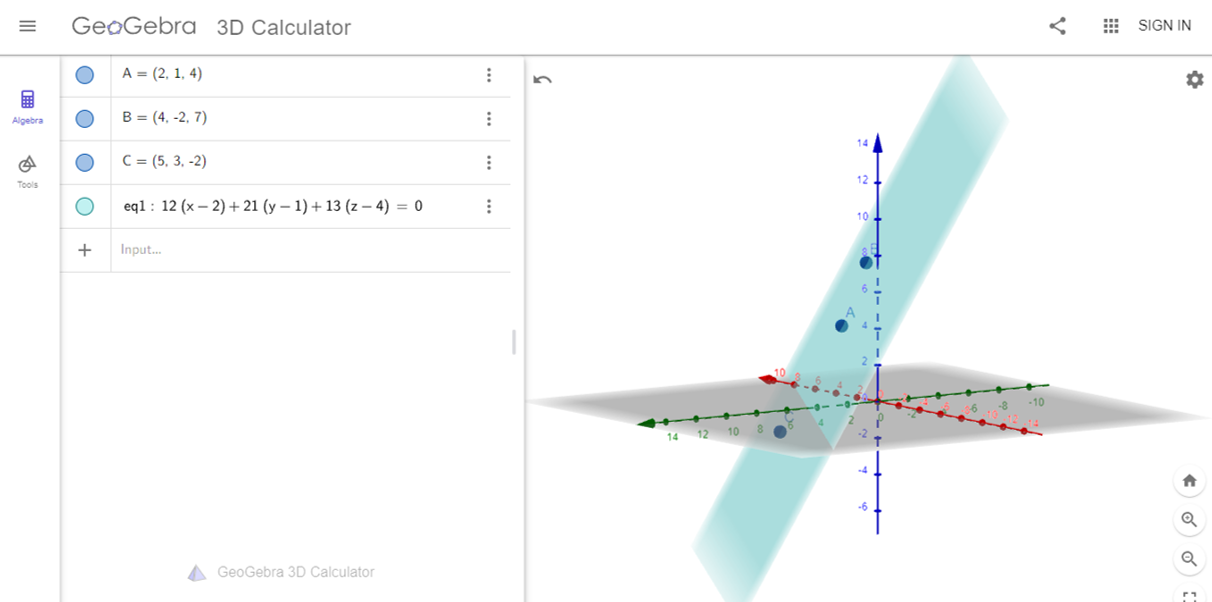
\includegraphics[width=1\textwidth]{3d-graph-worked(1).png}
\caption{3D Sketch of $12x+21y+13z = 97$ with points $P(2,1,4)$ and $Q(4,-2,7)$ and $R(5,3,-2)$}
\label{fig:Plane_3D_worked_1}
\end{figure}



\subsubsection{Finding out if 3 points are collinear in 3-Space}
Problem statement: Show that the points $A(1,2,3) , B(3,8,1), C(7,20,-3)$ are collinear. \\

Methodolgy: \\

First we need to find the vectors $\vec{AB}$ and $\vec{AB}$ and see if there is any relation/ratio between them.\\

$\vec{AB} = \left\langle 3-1,8-2,1-3\right\rangle = \left\langle 2,6,-2\right\rangle$ \\

$\vec{AC} = \left\langle 7-1,20-2,-3-3\right\rangle = \left\langle 6,18,-6\right\rangle$ \\

as you can see $\vec{AC} = 3\vec{AB}$ \\

$\therefore$ the points $A,B,C$ are collinear.

For fun let me show you how this looks in 3D.

\begin{figure}[H]
\centering
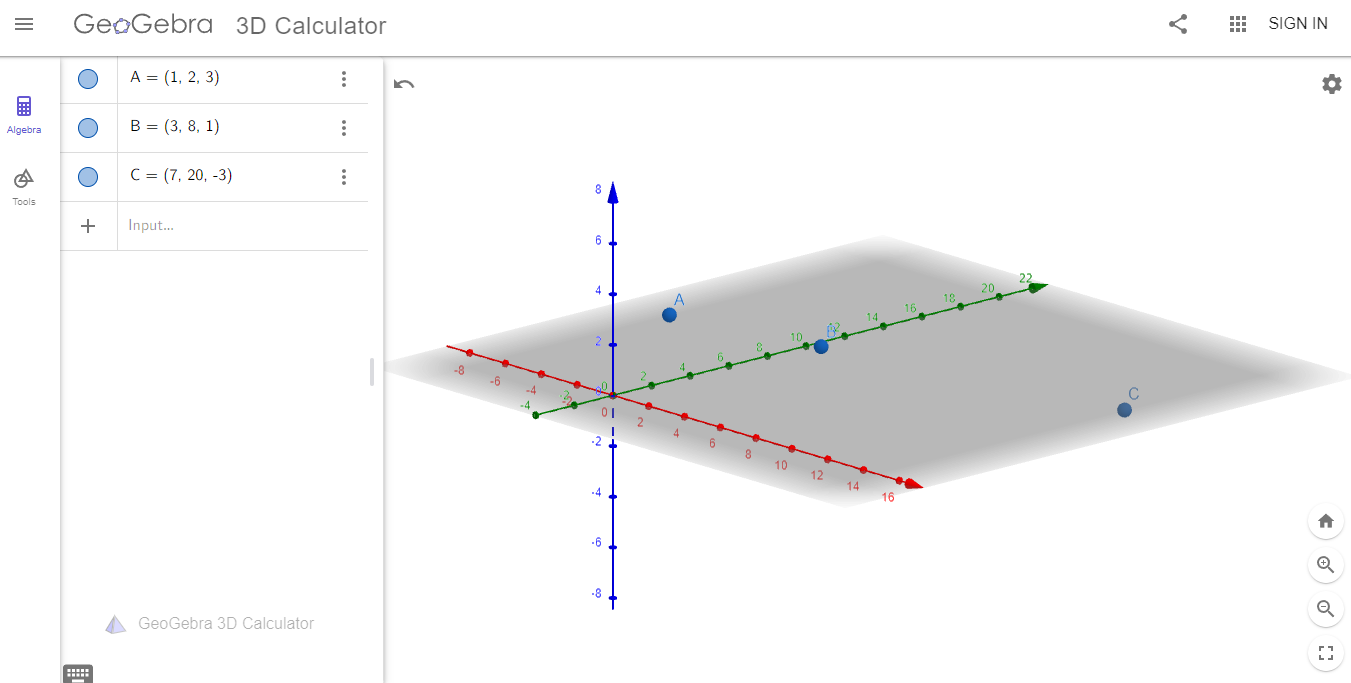
\includegraphics[width=1\textwidth]{3d-graph-worked(2).png}
\caption{3D Sketch of $A(1,2,3) , B(3,8,1), C(7,20,-3)$}
\label{fig:Plane_3D_worked_2}
\end{figure}

\subsubsection{Determining if two planes are parallel}
Problem statement: Determine if $L \land V$ are parallel. \\ 

Given: \\

\[ L
\begin{cases} 
x = 3t \\ 
y = 1+2t & -\infty < t < \infty \\ 
z = 2-t \\
\end{cases} 
\]

$V$ is a plane in 3-space defined by the equation: \\
\begin{center}
$V: 4x-y+2z=1$
\end{center}

Methodolgy: \\

Let $n = (4,-1,2)$ and $v = (3,2,-1)$ this is taken from the $(a,b,c)$ of the plane equations. \\

Since $L$ is a line in 3-space, $n$ is a normal of $V$ and we can consider $v$ parallel to $L$

\begin{figure}[H]
\centering
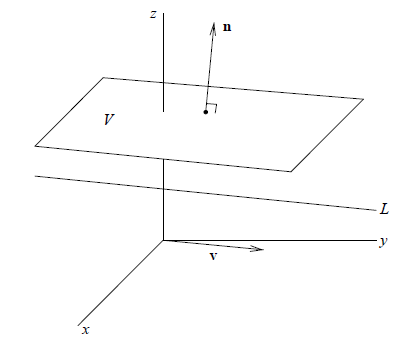
\includegraphics[width=0.5\textwidth]{sketch-3d-3.png}
\caption{3D Sketch of $L \land V$}
\label{fig:Plane_3D_worked_3}
\end{figure}

Now to find out if $V$ is parallel to $L$ we check if $n$ and $v$ dot product is 0 and perpendicular to each other. \\

$\vec{n}\cdot \vec{v} = (3,2,-1)*(4,-1,2)$ \\

$= 12-2-2 $ \\

$= 8$ \\

Hence $v$ is not perpendicular to $n$ and hence $L$ is not parallel to $V$.

\subsubsection{Finding the equation of a lane which contains a line and is perpendicular to another plane}
Problem statement: Find an equation for the plane $V_2$ which contains $L$ and is perpendicular to $V_1$:

Given: \\

\[ L
\begin{cases}
x = -1+3t \\
y = 5+2t & -\infty < t < \infty \\
z = 2-t \\
\end{cases}
\]

and $V_1$ is the plane in 3-space defined by: \\
\begin{center}
$V_1: 2x-4y+2z=9$
\end{center}

Procedure: \\

$L$ is given in vector form $(x,y,z) = (-1,5,2) + (3,2,-1)t$ \\ 

Hence $P = (-1; 5; 2)$ is a point on $L$ and $v = (3; 2;-1)$ is a vector parallel to $L$: Since $V_2$ contains $L$ it
follows that $P = (-1; 5; 2)$ is a point in $V_2$ and $v = (3; 2;-1)$ is parallel to $V_2$:
From the equation of $V_1$ it follows that a vector perpendicular to $V_1$ is $n_1 = (2;-4; 2)$ :
Since $V_1$ is perpendicular to $V_2$ it follows that $n_1 = (2;-4; 2)$ is parallel to $V_2$:

\begin{figure}[H]
\centering
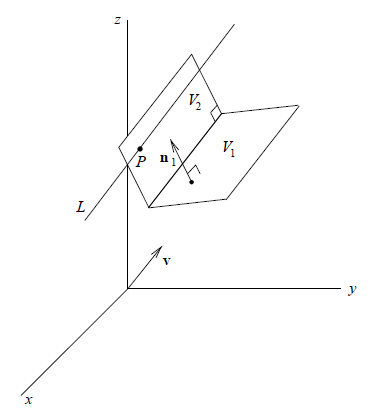
\includegraphics[width=0.5\textwidth]{sketch-3d-4.png}
\caption{3D Sketch of $L \land V_1 \land V_2$}
\label{fig:Plane_3D_worked_4}
\end{figure}

Thus $v$ and $n_1$ are parallel to $V_2$. \\

Thus $n_2 = v \times n_1$ is a vector perpendicular to $V_2$:

Computing the cross product of $v$ and $n_1$: \\ 

Using: \\

$\left(u_1,\:u_2,\:u_3\right)\times \left(v_1,\:v_2,\:v_3\right)=\left(u_2v_3-u_3v_2,\:u_3v_1-u_1v_3,\:u_1v_2-u_2v_1\right)$ \\

We get the vector $n_2$: \\

$= \begin{pmatrix}2\cdot \:2-\left(-1\cdot \left(-4\right)\right)&-1\cdot \:2-3\cdot \:2&3\left(-4\right)-2\cdot \:2\end{pmatrix}$ \\


$= \begin{pmatrix}0&-8&-16\end{pmatrix}$ \\

Factoring the vector: \\

$= -8(0,1,2)$ \\

Hence $n = (0,1,2)$ is a vector perpendicular to $V_2$ \\

Thus $V_2$ is a plane containing the point $P = (-1; 5; 2)$ and a normal to $V_2$ is $n = (0; 1; 2)$ : \\

$\therefore V_2$ is defined by: \\

$V_2: 0(x + 1) + 1 (y - 5) + 2 (z - 2) = 0$ (point-normal) \\

expanding it will give: \\

$V_2 = y+2z-9=0$ \\

Verifying if we got the correct calculations lets plot everything in 3-Space:

\begin{figure}[H]
\centering
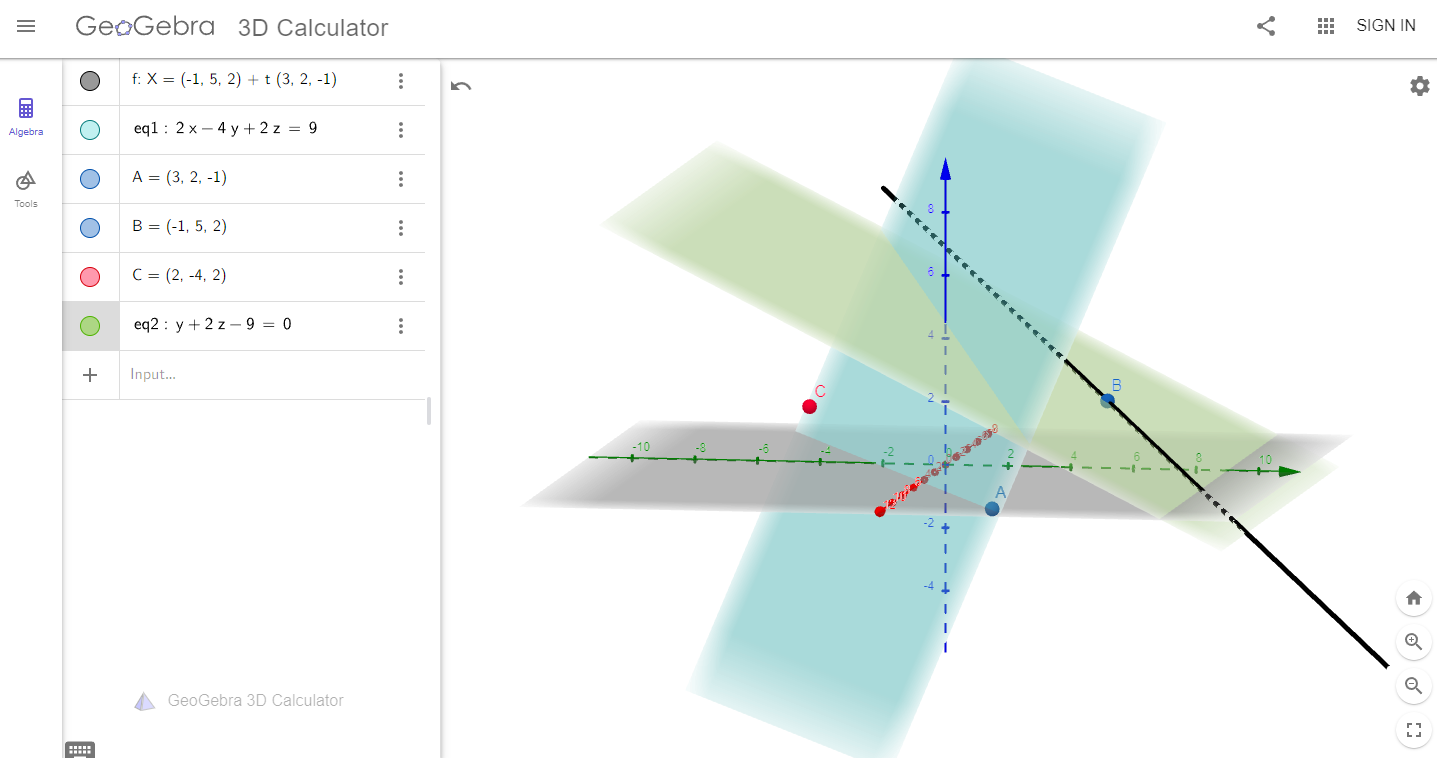
\includegraphics[width=1\textwidth]{sketch-3d-5.png}
\caption{3D Graph of $L \land V_1 \land V_2 \land $} some vectors.
\label{fig:Plane_3D_worked_5}
\end{figure}

\subsubsection{Calculating distance between a point and a plane}

Problem statement: Calculate the distance between a point and a plane. \\

Given: \\

$Z(2,5,10)$ \\

$V_1: 2x-4y+2z=9$ \\

Methodology: \\

We use the distance formula denoted by: \\

$d = \frac{Ax_0+By_0+Cz_0+D}{\sqrt{A^2+B^2+C^2}}$ \\

$d = \frac{(2(2)-4(5)+2(10)-9)}{\sqrt{2^2+4^2+2^2}}$ \\

$\therefore d = -1.02$ \\

\subsubsection{Finding point-normal form of an equation passing passing via point and having a given normal}

Problem statement: Find the point-normal form of an equation passing through a point and having a given normal. \\

Given: \\

$P(2,5,10)$ \\

$\vec{v}  = (0,1,2)$ \\

Methodology: \\ 

Subsitute equation using the given structure: \\

Using format $a(x - x_0) + b(y - y_0) + c(z - z_0) = 0$ \\

$\therefore (y-5) + 2(z-10) = 0$ \\

Our final equation is: \\ 

$y+2z-25$ \\

Our graph looks like this: \\

\begin{figure}[H]
\centering
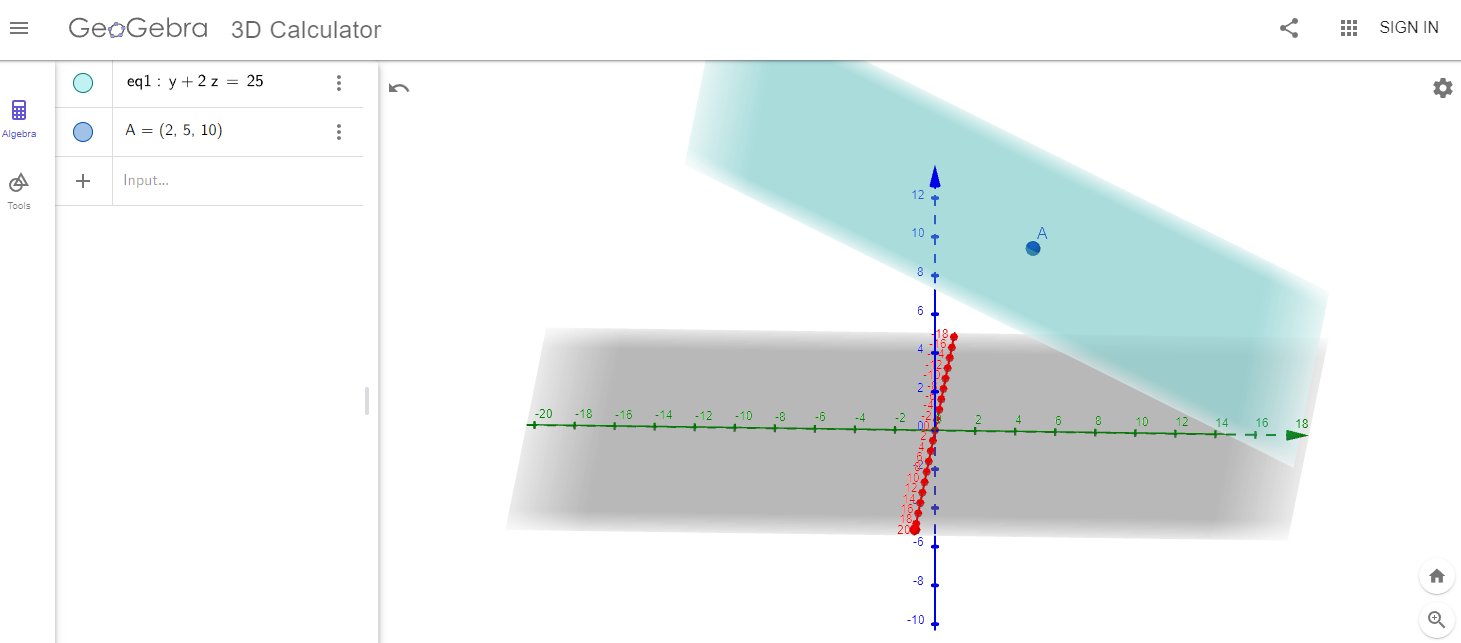
\includegraphics[width=1\textwidth]{sketch-3d-6.png}
\caption{3D Graph of $P=A \land y+2z-2$}
\label{fig:Plane_3D_worked_6}
\end{figure}

\subsubsection{Finding parametric equations for intersecting planes}

Problem statement: Find the parametric equations for intersecting planes. \\

Consider:

\[
\begin{cases}
V_1: 2x-4y+2z=9 \\
V_2: 1x-3y+5z=24 \\
\end{cases}
\]

In order to find our directional vector we need to find the intersection of the two planes. \\

To get started we set $z=0$ \\

Now we get a new system: \\

\[
\begin{cases}
V_1: 2x-4y=9 \\
V_2: 1x-3y=24 \\
\end{cases}
\]

Solve for $x$ and $y$ \\

$x = \frac{-69}{2} \land y = \frac{-39}{2}$ \\

so our $\vec{r}$ positional vector is: \\

$\vec{r} = (\frac{-69}{2},\frac{-39}{2},0)$ \\ 

Now work out our directional vector/cross product of $V_1$ and $V_2$: \\

our cross product is: \\

$\begin{pmatrix}2&-4&2\end{pmatrix}\times \begin{pmatrix}1&-3&5\end{pmatrix}=\begin{pmatrix}-14&-8&-2\end{pmatrix}$ \\

$\therefore$ our line can be described by: \\

$L =  (\frac{-69}{2},\frac{-39}{2},0)+(-14,-8,-2)t$  \\

Our graph looks like this: \\

\begin{figure}[H]
\centering
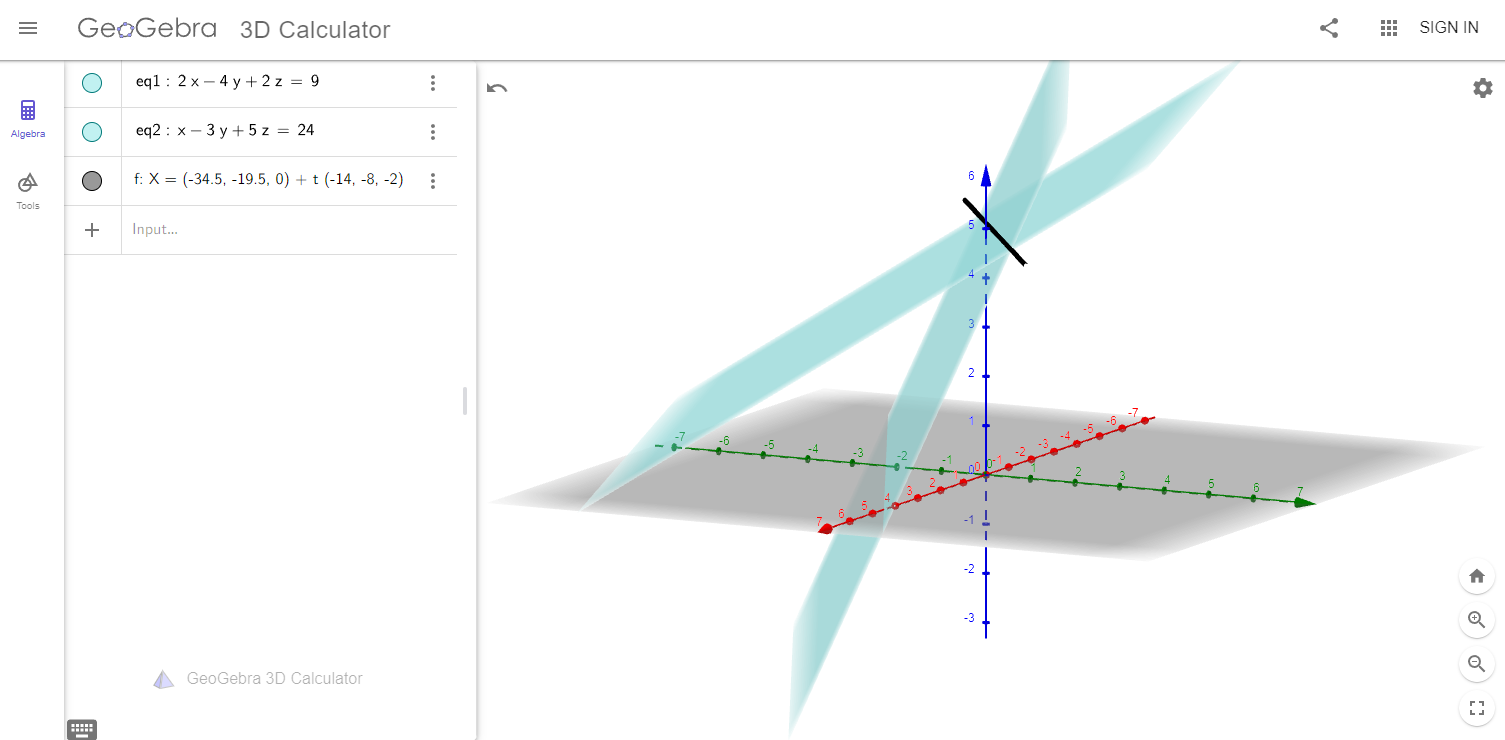
\includegraphics[width=1\textwidth]{sketch-3d-7.png}
\caption{3D Graph of  $V_1 \land V_2 \land L = (\frac{-69}{2},\frac{-39}{2},0)+(-14,-8,-2)t$}
\label{fig:Plane_3D_worked_7}
\end{figure}